\documentclass[11pt]{article} 
\usepackage{geometry}
\usepackage{bm}
% \geometry{left=2cm,right=2cm,top=1cm,bottom=2cm}
\usepackage{simpleConference}
\usepackage{times}
\usepackage{graphicx}
\usepackage{amssymb}
\usepackage{url,hyperref}

\usepackage{booktabs} 
\usepackage{amsfonts}  
\usepackage{amsmath}
\usepackage{float}
\usepackage{subfigure}
\usepackage{setspace}
\renewcommand{\baselinestretch}{1.0}

\usepackage[sort]{natbib}  % 引文格式
\usepackage{multicol}
\usepackage{multirow}
\usepackage{setspace} % 可设置表格行高
% \usepackage[colorlinks, linkcolor=blue]{hyperref} % 超链接
\usepackage{float} %图片紧跟文字
\usepackage{subfigure}
\usepackage{algorithm}
\usepackage{algorithmic}
\renewcommand{\algorithmicrequire}{ \textbf{Input:}}
\renewcommand{\algorithmicensure}{ \textbf{Output:}}
\usepackage{array}
% set page geometry
% \usepackage[verbose=true,letterpaper]{geometry}
\AtBeginDocument{
  \newgeometry{
    textheight=9in,
    textwidth=6.8in,
    top=1in,
    headheight=14pt,
    headsep=25pt,
    footskip=30pt
  }
}

% \widowpenalty=10000
% \clubpenalty=10000
% \flushbottom
% \sloppy

\usepackage{fancyhdr}
\pagestyle{fancy}
\lhead{} 
\rhead{} 
\chead{\bfseries CIE6010 Final Report} % CIE6036 Project Report
% \lfoot{} 
\cfoot{\thepage}
% \rfoot{\thepage} 
\renewcommand{\headrulewidth}{0.4pt} 
% \renewcommand{\footrulewidth}{0.4pt}
\usepackage[font=small,labelfont=bf]{caption}


\begin{document}

\title{Minimum Surfaces and Obstacle Problems}

% \author{Yu Fangchen, Cai Weilin, Li Chi, Chen Weibin \\
% 	\and
% 	Department of Computer and Information Engineering\\
% 	The Chinese University of Hong Kong, Shenzhen \\ \\
% 	\today
% }

\author{
	Cai Weilin \\
	\texttt{220019066@link.cuhk.edu.cn} \\
	\and
	Li Chi \\
	\texttt{220019044@link.cuhk.edu.cn} \\
	\and
	Department of Computer and Information Engineering\\
	The Chinese University of Hong Kong, Shenzhen \\ \\
	\today
}

\maketitle

\small


\begin{abstract}
% TODO Change Dynamic Programming into other expression (important) .
Minimum surfaces and obstacle problems are well-defined to determine the surface with minimal area that lies above an obstacle with given boundary conditions. In this report, we first formulate a unconstrained minimum surface problem without considering obstacles, and then addtional obstacle constraints are introduced to construct a constrained optimization problem. Besides, an example of the problem is given and solved with a linear finite-dimensional minimization method via a discretization scheme. Firstly, we triangulate the domain of definition, and then approxiamte the objective by a piecewise linear function on each triangle considering both boundary and obstacle constraints. Here, we introduce several efficient algorithms, including unconstrained and constrained optimization methods, for tackling the pre-defined problem. Also, we analyze the perfomance of each proposed method as well as different parameter choices in boundary function and discretization degree. Lastly, we discuss and conclude our observations and results when implementing different optimization methods for different problems in depth.

\end{abstract}
%\keywords{Minimum surface \and Obstacle problem \and Finite element approximation \and Nonlinear programming}

\section{Introduction}
The minimum surfaces and obstacle problems aim to generate a two dimensional surface of minimal area with a given closed curve in $\mathbb R^{3}$ as boundary \cite{dolan2004benchmarking}. It's regarded as a classic motivating example in the mathematical area of variational inequalities and free boundary problems, and widely applided to the domain of physics, biology, financial mathematics and optimal control \cite{zosso2017efficient,ros2018obstacle,caffarelli1998obstacle}. In \cite{ros2018obstacle}, the author classisifies the obstacle problems with free boundary into three categories: classical obstacle problem, the thin obstacle problem and obstacle problems for integro-differential operators. Meanwhile, he describles comprehensively the classical regularity theory for the defined obstacle problem and with its applications in such areas. In recent years, some efficent and advanced methodologies, such as sequencial quadratic programming \cite{liu2009solution}, primal-dual method \cite{zosso2017efficient} and PDE accelerations \cite{calder2019pde} have been proposed to solve these obstacle problems. The classical formulation can be represented as follows. Suppose that the surface can be showed in nonparametric form $z:\mathbb R^{2} \rightarrow$ $\mathbb R,$ and the requirement is $z \geq z_{L}$ for some obstacle $z_{L} .$ The solution of this obstacle problem minimizes the function $f: K \rightarrow \mathbb R$
$$
f(z)=\int_{D} \sqrt{1+\|\nabla z(x)\|^{2}} d x \eqno(1)
$$
over the convex set
$$
K=\left\{z \in H^{1}(D) \mid z(x)=z_{D}(x) \text { for } x \in \partial D, z(x) \geq z_{L}(x) \text { for } x \in D\right\}  \eqno(2)
$$
where $\|\bullet\|$ represents the Euclidean norm, $H^{1}(D)$ is the space of functions with gradients in $L^{2}(D) .$ The function $z_{D}: \partial D \rightarrow \mathbb R$ defines the boundary data, and $z_{L}:D \rightarrow \mathbb R$ is the obstacle. We assume that $z_{L} \leq z_{D}$ on the boundary $\partial D$.

In this project, we first construct a unconstrined optimization problem by only considering minimal surface problems for a special issue. Subsequently, obstacle constraints will be introduced to complete the whole model formulation. Several effective unconstrained and constrained algorithms will also be implemented to test the perfomance for different defined problems. We then summarize and conclude our main results and observations for these experiments. 

The reminder of the report is organized as follows. Section 2 gives a description and mathematicla formualtion for these two problems. Section 3 describes our utilized unconstrained and constrained algorithms. In Section 4, we compare and analyze the results of these methods. Section 5 presents in-depth discussion on a variety of numerical experiments. We conclude in Section 6 with some future works.
\section{Mathematic Model}
In this part, we describe the minimum surfaces and obstacles problems in Section 2.1 and formulate them mathematically in Section 2.2.
\subsection{Model Description}
\subsubsection{Minimum Surfaces}
The minimum surface problem is to generate a two dimensional surface that is defined on a set $\Omega \subset \mathbb{R}^{2}$ only from data and observations given at the boundary of $\Omega.$ In particular, let $\Gamma=\partial \Omega$ denote the boundary of the set $\Omega$ and let $r: \Gamma \rightarrow \mathbb{R}$ be a given function on $\Gamma .$ Then, we will solve a discretized, finite-dimensional minimization task to find a function $q: \operatorname{cl} \Omega \rightarrow \mathbb{R}$ satisfying the following goals:

\begin{itemize}
    \item $ q(t)=r(t) \quad \forall t \in \Gamma$.
    \item The graph of $q$ has minimum surface.
\end{itemize}
\subsubsection{Obstacle Problems}
The minimum surface problem could be further extended into obstacle problems, which means the reference set $\Omega$ contains additional obstacles that need to be considered when building the function $q$. As shown previously, the boundary set $\Gamma=\partial \Omega$ and boundary function $r: \Gamma \rightarrow \mathbb{R}$ are the same as minimum surface problem. Moreover, let $\mathcal{B} \subset \Omega$ be an obstacle set and let $b: \mathcal{B} \rightarrow \mathbb{R}$ be a given obstacle function. Here, we will utilize different approaches to solve the constrained problem under different types of obstacles, to find a function $q: \operatorname{cl} \Omega \rightarrow \mathbb{R}$ satisfying the following goals:
\begin{itemize}
  \item $ q(t)=r(t) \quad \forall t \in \Gamma$. 
  \item $ q(t) \geq b(t) \quad \forall t \in \mathcal{B} $.
  \item The graph of $q$ has minimum surface.
\end{itemize}



\subsection{Model Formulation}
\subsubsection{Minimum Surfaces}
In order to solve the problem numerically, we utilize a discretized triangulating scheme to express the problem as a minimization task over the space of piecewise linear functions. In \cite{shen1992finite}, the linear finite dimensional approximation for the minimal surface with obstacle is analyzed while the existence and uniqueness of the solution for the discrete problem are shown, and meanwhile the error estimate of the approximation methodology is also obtained. 

In this case, we follow the process of trianglation and our objective is transformed to find a function  $q: \operatorname{cl} \Omega \rightarrow \mathbb{R}$ via solving a minimization problem in the finite discretized approximation scheme. As shown in figure 1, we first assume that $\Omega=\left(a_{1}, b_{1}\right) \times\left(a_{2}, b_{2}\right)$ has a simple rectangular shape with $a_{1}<b_{1}, a_{2}<b_{2},$ and $a_{i}, b_{i} \in \mathbb{R}, i \in\{1,2\} .$ And then generate a regular grid with $m \cdot n$ nodes $t_{11}, \ldots, t_{1 n}, t_{21}, \ldots, t_{(m-1) n}, t_{m 1}, \ldots, t_{m n} \in \mathbb{R}^{2}$
covering the set cl $\Omega$ while three neighboring nodes can form one of the triangles $T_{k} .$ Using a triangulation $\operatorname{cl} \Omega=\bigcup_{k=1}^{\kappa} T_{k}$, we then approximate and discretize $\operatorname{cl} \Omega$.
\begin{figure*}[htbp]
  \centering
  \caption{Illustration of the discretization scheme}
  \label{fig:discretization_scheme}
\end{figure*}

In particular, we set $\Omega=(0,1) \times(0,1) \in \mathbb R^{2}$ and $\Gamma=\partial \Omega$. Using triangulation, the set $\operatorname{cl} \Omega$ is discretized to $2 n^{2}$ triangles, with each point $t_{i, j}=\left(\frac{i}{n}, \frac{j}{n}\right), i=0,1, \ldots, n, j=0,1, \ldots, n .$ Our piecewise linear function $q_{T}: \mathrm{cl} \Omega \rightarrow \mathbb{R}$ is uniquely characterized by its node values:
$$
q_{T}\left(t_{i j}\right)=x_{i, j} \quad \forall i, j=0, \ldots, n  \eqno(3)
$$
along the boundary $\Gamma$, we have 
$$
q_{T}\left(t_{i j}\right)=x_{i j}=r\left(t_{i j}\right) \quad \forall t_{i j} \in \Gamma  \eqno(4)
$$

It's clear that $q_{T}$ builds a mapping from the set $\Omega$ to $\mathbb{R},$ which is an approximation of the two-dimensional surface.
Therofore, our goal is to determine these $X$ such that the surface area of these triangles on cl $\Omega$ has minimum value.Thus, the full optimization problems is given as below:
$$
\min _{X=\left(x_{i, j}\right) \in \mathbb{R}^{n \times n}} f(X)=\sum_{k=1}^{\kappa} A_{k}(X) \qquad \text { s.t. } \quad x_{i, j}=r\left(t_{i j}\right) \ \forall t_{i j} \in \Gamma  \eqno(5)
$$
Where $A_{k}(X)$ denotes the area of the triangle $T_{K},$. Moreover, the corresponding decision variables can be diminished into $X=\left(x_{i, j}\right), i=1,2, \ldots, n-1$, $j=1,2, \ldots, n-1$
since the value of $q_{T}$ on the boundary is given, we can omit these variables. Therefore, this optimization problem can be transferred into an unconstrained problem:
$$
\min _{X=\left(x_{i, j}\right) \in \mathbb{R}^{(n-1) \times(n-1)}} f(X)=\sum_{k=1}^{\kappa} A_{k}(X)  \eqno(6)
$$
With this regard, we treat $x_{i, j}, i \in\{0, n\}$ or $j \in\{0, n\}$ as known parameters. Hence, we can implement unconstrained optimization algorithms to solve the minimum surfaces problem.
\subsubsection{Obstacle Problems}
We can also utilize the same discretization scheme and triangulation technique as presented in minimum surface problems to approximate the target set $\operatorname{cl} \Omega$ and the function $q$ while satisfying the obstacle constraints. This is equivalent to 
$$
x_{i j} \geq b\left(t_{i j}\right) \quad \forall t_{i j} \quad \text { with } \quad t_{i j} \in \mathcal{B}  \eqno(7)
$$
then the obstacle problem can be represented as follows:
$$
\min _{X=\left(x_{i j}\right) \in \mathbb{R}^{m \times n}} \sum_{k=1}^{\kappa} A_{k}(X) \quad \text { s.t. } \quad\left[\begin{array}{ll}
x_{i j}=r\left(t_{i j}\right) & \forall t_{i j} \in \Gamma \\
x_{i j} \geq b\left(t_{i j}\right) & \forall t_{i j} \in \mathcal{B}
\end{array}\right.  \eqno(8)
$$



\section{Approach}
In this part, we will employ several unconstrained and constraints algorithms for 






\subsection{Unconstrained Optimization Algorithms}
\begin{algorithm}[H]
  \caption{Gradient Descent Method (with Backtracking)}
  \label{alg:Gradient}
  \begin{algorithmic}[1]
  \REQUIRE
  Initial point $x^{0}$
  \STATE For $k=0,1, \ldots$ \\
  \STATE Choose stepsize $\alpha^{k}$ by backtracking. \\
  \STATE $x^{k+1}=x^{k}-\alpha^{k} \nabla f\left(x^{k}\right)$. \\
  \STATE Stop if $\left\|\nabla f\left(x^{k+1}\right)\right\| \leq \epsilon$. \\     
  \ENSURE $x^{k+1}$ 
 \end{algorithmic}
 \end{algorithm} 
 
 \begin{algorithm}[H]
   \caption{Globalized Newton Method}
   \label{alg:Newton}
   \begin{algorithmic}[1]
   \REQUIRE
   Initial point $x^{0}, \beta_{1}, \beta_{2}, p$
   \STATE For $k=0,1, \ldots$ \\
   \STATE Compute the Newton direction $s^{k}$ by solving $\nabla^{2} f\left(x^{k}\right) s^{k}=-\nabla f\left(x^{k}\right)$. \\
   \STATE If $-\nabla f\left(x^{k}\right)^{\mathrm{T}} s^{k} \geq \min \left\{\beta_{1}, \beta_{2}\left\|s^{k}\right\|^{p}\right\}\left\|s^{k}\right\|^{2}$, then set $d^{k}=s^{k}$. Otherwise set $d^{k}=-\nabla f\left(x^{k}\right)$. \\
   \STATE Choose stepsize $\alpha^{k}$ by backtracking. \\  
   \STATE $x^{k+1}=x^{k}+\alpha^{k} d^{k}$. \\
   \STATE  Stop if $\left\|\nabla f\left(x^{k+1}\right)\right\| \leq \epsilon$. \\  
   \ENSURE $x^{k+1}$ 
  \end{algorithmic}
  \end{algorithm} 
 
 
 
 
 
 \begin{algorithm}[H]
   \caption{L-BFGS Method}
   \label{alg:L-BFGS}
   \begin{algorithmic}[1]
   \REQUIRE
 Initial point $x^{0}, B_{0}$ \\
   \STATE For $k=0,1, \ldots$ \\
   \STATE Compute the quasi-Newton direction $d^{k}$ by solving $B_{k} s^{k}=-\nabla f\left(x^{k}\right), x^{k+1}=x^{k}+s^{k}$. \\
   \STATE $\quad$ Stop if $\left\|\nabla f\left(x^{k+1}\right)\right\| \leq \epsilon$. \\
   \STATE Set $y^{k}=\nabla f\left(x^{k+1}\right)-\nabla f\left(x^{k}\right), B_{k+1}^{\text {BFGS }}=B_{k}+\frac{y^{k}\left(y^{k}\right)^{\top}}{\left(y^{k}\right)^{\top} s^{k}}-\frac{\left(B_{k} s^{k}\right)\left(B_{k} s^{k}\right)^{\top}}{\left(s^{k}\right)^{\top} B_{k} s^{k}}$ \\
   \ENSURE $x^{k+1}$ \\
   \end{algorithmic}
 \end{algorithm}
 
\subsection{Constrained Optimization Algorithms}

\begin{algorithm}[H]
  \caption{Quadratic Penalty Method}
  \label{alg:Penalty}
  \begin{algorithmic}[1]
  \REQUIRE
  Initial point $x^{-1}$, penalty parameter $\alpha_{0}>0$
  \STATE For $k=0,1, \ldots$ \\
  \STATE Compute the global solution $x^{k}$ of the penalty problem $\min _{x} P_{\alpha_{k}}(x)$. \\     
  \ENSURE Terminate if $x^{k} \in X$. Otherwise select $\alpha_{k+1}>\alpha_{k}$.  
 \end{algorithmic}
 \end{algorithm} 






 \begin{algorithm}[H]
  \caption{Projected Gradient Method}
  \label{alg:Projected}
  \begin{algorithmic}[1]
  \REQUIRE
  Initial point $x^{0} \in C, \sigma, \gamma \in(0,1)$
  \STATE For $k=0,1, \ldots$ \\
  \STATE $\quad$ Select $\lambda_{k}>0$ and compute $\nabla f\left(x^{k}\right)$ and the new direction $d^{k}=-F_{\lambda_{k}}\left(x^{k}\right)$.  \\
  \STATE $\quad$ If $\left\|d^{k}\right\| \leq \lambda_{k} \epsilon$, then STOP and $x^{k}$ is output.  \\
  \STATE Choose a maximal step size $\alpha_{k}$ by backtracking. \\    
  \STATE Set $x^{k+1}=x^{k}+\alpha_{k} d^{k}$
  %\ENSURE $x^{k+1}$ 
 \end{algorithmic}
 \end{algorithm} 



\subsection{Addtional Techniques}
In our experiment, we will explore four additional techniques (nonmonotone line search procedures, Barzilai-Borwein
steps, inertial techniques and momentum, compact representation of the L-BFGS update) to adjust and potentially accelerate our proposed  algorithm. 
Exact line search 
The Barzilai-Borwein (BB) method is a popular and efficient tool for solving large-scale unconstrained optimization problems \cite{raydan1997barzilai}. Its search direction is the same as for the steepest descent method, but its stepsize rule is different. Owing to this, it converges much faster than the steepest descent method \cite{burdakov2019stabilized}. The full implement process is showed in algorithm \ref{alg:BB method} as follows.

\begin{algorithm}[H]
  \caption{Barzilai and Borwein Gradient Method}
  \label{alg:BB method}
  \begin{algorithmic}[1]
  \REQUIRE
Initial point $x^{0},0<\varepsilon \ll 1 $ \\
  \STATE For $k=0,1, \ldots$ \\
  \STATE If $\left\|\nabla f\left(x^{k}\right)\right\| \leq \varepsilon,$ stop ; otherwise let $d_{k}=-\nabla f\left(x^{k}\right)$. \\
  \STATE If $k=0,$ find $\alpha_{0}$ by line search; otherwise compute $\alpha_{k}$ by 
  $
  \alpha_{k}=\frac{s_{k-1}^{T} y_{k-1}}{y_{k-1}^{T} y_{k-1}}
  $
  where $s_{k-1}=x_{k}-x_{k-1}, y_{k-1}=\nabla f\left(x^{k}\right)-\nabla f\left(x^{k-1}\right)$. \\
  \STATE Set $x_{k+1}=x_{k}+\alpha_{k} d_{k}$ \\
  \STATE $k:=k+1$, return to Step 1 \\
  \end{algorithmic}
\end{algorithm}

The compact representation of the quasi-Newton updating matrix is derived to the use in the form of limited memory update in
which the vector is replaced by a modified vector so that more available information about the function can be
employed to increase the accuracy of Hessian approximations. The global convergence of the proposed method is proved.





\section{Experiment Analysis}
In this part, we will implement several unconstrained and constrained optimization alogorithms to solve minimum surfaces and obstacle problems respectively. More specificly, we will employ 3 basic unconstrained optimization algorithms (gradient descent method with backtracking, globalized Newton method, L- BFGS method) with 5 different boundary functions in the minimum surface problems. We will also consider how the discretization degree and addtional techniques influence our experimental results. For the obstacle problem, we will apply two constrained optimization algorithms (quadratic penalty method and projected gradient method) in combination with different obstacle functions. And meanwhile, we will analyze the perfomance of different implemented algorithms and discuss some potential improvements.
\subsection{Minimum Surfaces}
At first, we will illustrate five different boundary functions. Then we will choose one advanced algorithm to solve the minimum surface problem with five boundary functions and different discretization degree. Subsequently, we utilize other unconstrained optimization alogorithms and compare their perfomance from the perspective of relative objective function gap and iteration of norm of gradients. Finally, additional techniques such as exact line search, Barzilai-Borwein steps and inertial techniques will be introduced to accelerate the convergence process.
\subsubsection{Boundary Functions}
Here, figure \ref{fig:boundary} presents five different boundary function mentioned in the report requirement document. We will then determine the minimum surfaces using different boundary functions via our proposed algorithms.
\begin{figure}[!htbp]
    \centering
    \subfigure[$ r_1(x, y)=1+\sin (2 \pi x)$]
    {
    \centering
    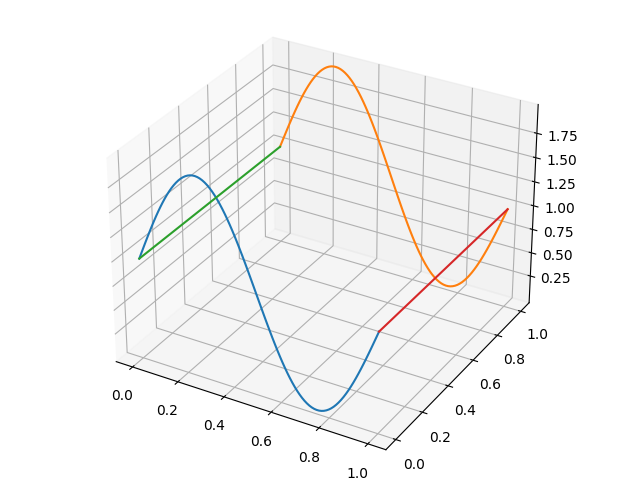
\includegraphics[width=0.3\columnwidth]{images/boundary/sin.png}
    }
    \subfigure[$ r_2(x, y)=1+\cos (1 / (x+0.001) )$]
    {
    \centering
    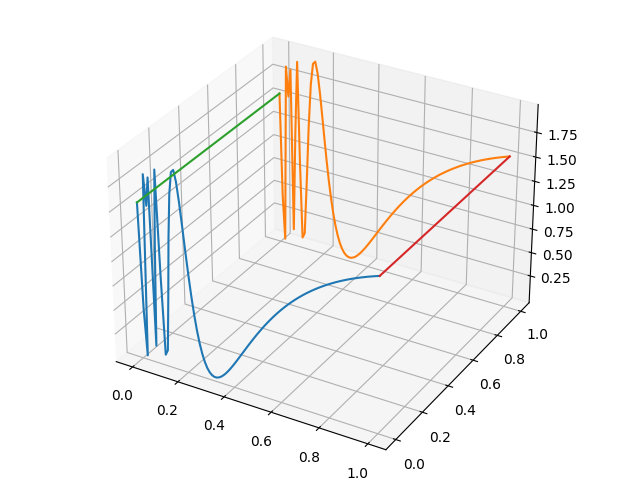
\includegraphics[width=0.3\columnwidth]{images/boundary/cos.png}
    }
    \subfigure[$ r_3(x, y)=\frac{1}{2}-\left|y-\frac{1}{2}\right|$]
    {
    \centering
    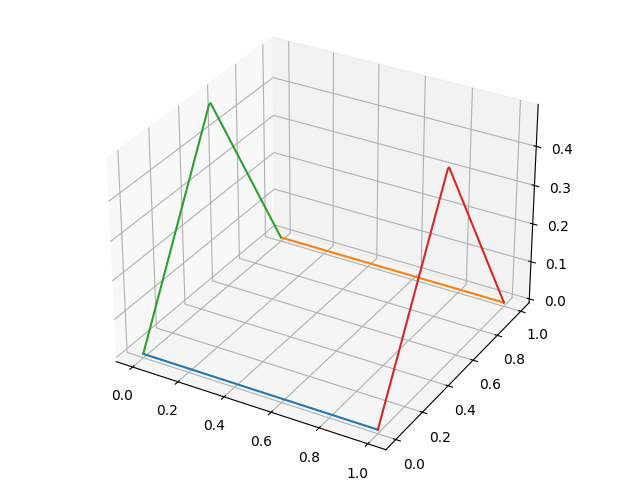
\includegraphics[width=0.3\columnwidth]{images/boundary/abs.png}
    }
    \subfigure[$ r_4(x, y)=(1+\exp (x y))^{-1}$]
    {
    \centering
    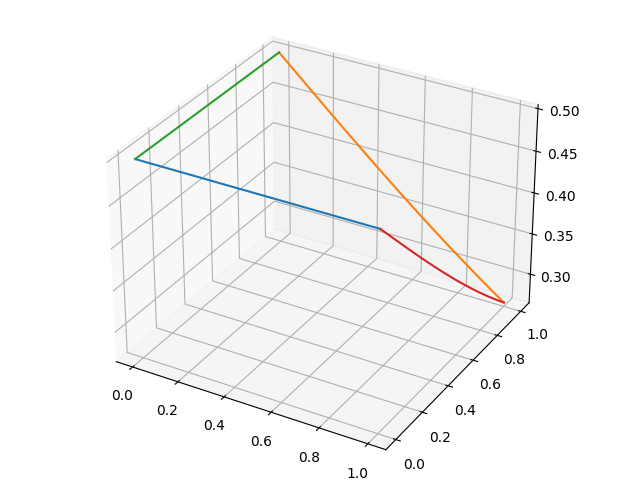
\includegraphics[width=0.3\columnwidth]{images/boundary/exp.png}
    }
    \subfigure[$ r_5(x, y)=1+\arcsin (-1+2 \sqrt{x y})$]
    {
    \centering
    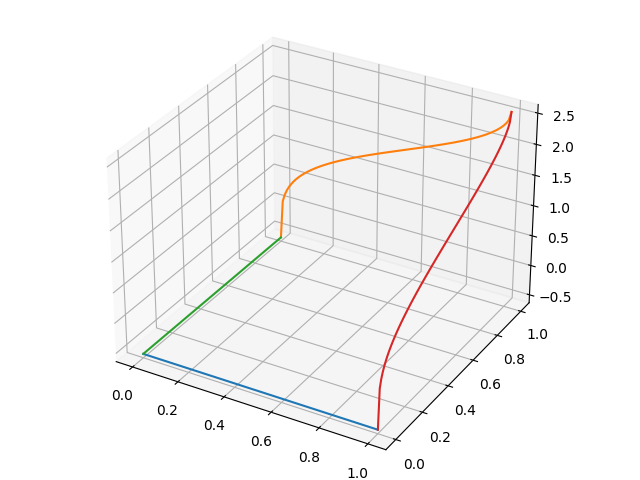
\includegraphics[width=0.3\columnwidth]{images/boundary/asin.png}
    }
    \caption{Five Boundaries in the Minimal Surface Problem (n=100)}
    \label{fig:boundary}  
\end{figure}
\subsubsection{Minimum Surface Results}
In order to demonstrate how the boundary function and discretization degree influence the minimal surface area, we choose globalized newton method to test these effects.

Comparing the corresponding subfigures between figure \ref{fig:boundary} and figure \ref{fig:min_surf_boundaries}, we can intuitively find out how the minimum surface come into shape. In order to control convariate, we choose $n=9$ and then generate the minimum surfaces under different boundaries. 

The minimal surface area depends on the number of the grid points. Figure \ref{fig:min_surf_discretization} shows how the discretization degree affect the formulation of minimum surface. It can be seen that the minimum surface becomes more and more smooth with larger discretization degree. As represented in table \ref{tab:per_vs_dis}, with the increase of the number of grid points, the minimal area is decreasing on the whole. With reference to the principle of calculus, we know the approximate error will be reduced with more grid points.In addition, with the increase of the number of discretization degree, the number of the variable is increasing, so the computation becomes slower and the iteration number also increases. 



\begin{table}[!ht]
    \caption{Perfomance Analysis with Different Discretization Degree}\label{tab:per_vs_dis}
    \begin{tabular*}{\hsize}{@{}@{\extracolsep{\fill}}cccc@{}}
    \toprule
             &Iteration number  &Final objective function  &Cost time(s)  \\
    \midrule
    $n=5$   &6   &2.4897  &0.371  \\
    $n=7$   &5   &2.4514  &0.752  \\
    $n=9$   &11  &2.4359  &2.855  \\
    $n=13$  &12  &2.4237  &7.152  \\
    $n=15$  &13  &2.4210  &10.868 \\
    $n=18$  &15  &2.4140  &18.741 \\
    \bottomrule
    \end{tabular*}
\end{table}

\begin{figure}[!htbp]
    \centering
    \subfigure[$ r_1(x, y)=1+\sin (2 \pi x)$]
    {
    \centering
    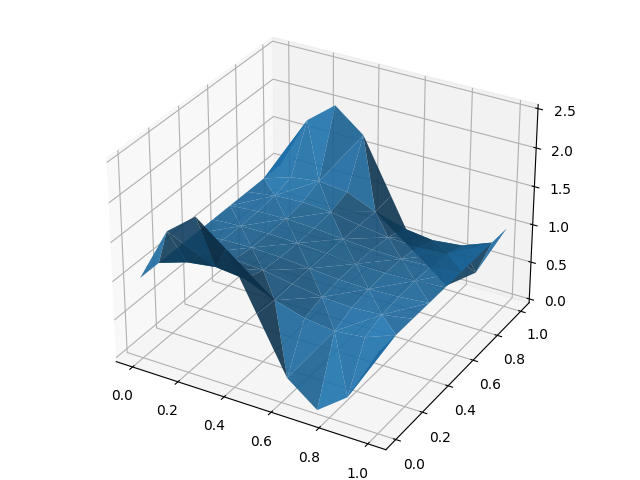
\includegraphics[width=0.3\columnwidth]{images/simple/min_surf_r0.png}
    }
    \subfigure[$ r_2(x, y)=1+\cos (1 / (x+0.001) )$]
    {
    \centering
    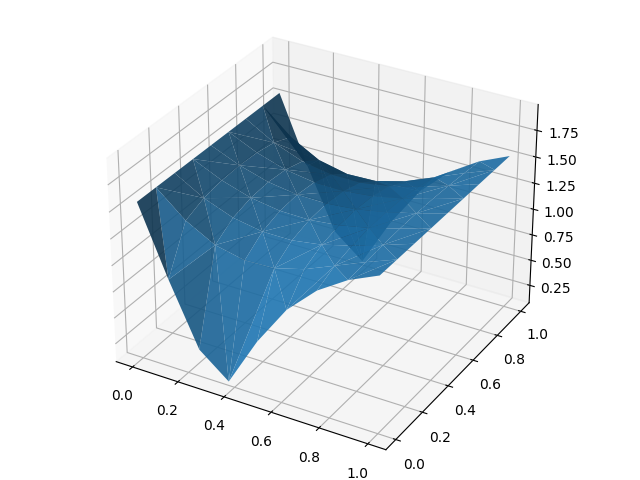
\includegraphics[width=0.3\columnwidth]{images/simple/min_surf_r1.png}
    }
    \subfigure[$ r_3(x, y)=\frac{1}{2}-\left|y-\frac{1}{2}\right|$]
    {
    \centering
    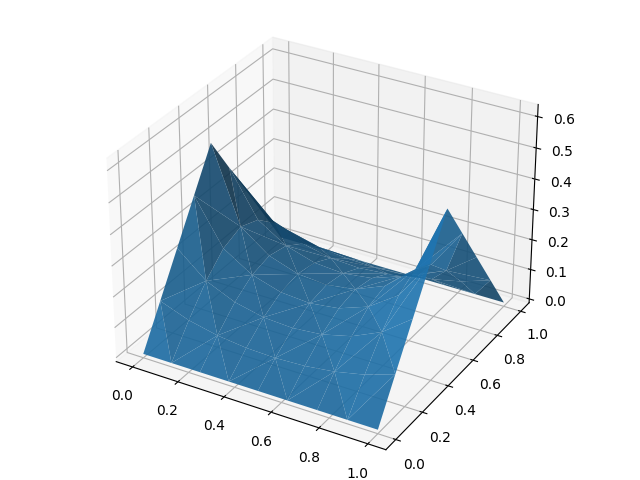
\includegraphics[width=0.3\columnwidth]{images/simple/min_surf_r2.png}
    }
    \subfigure[$ r_4(x, y)=(1+\exp (x y))^{-1}$]
    {
    \centering
    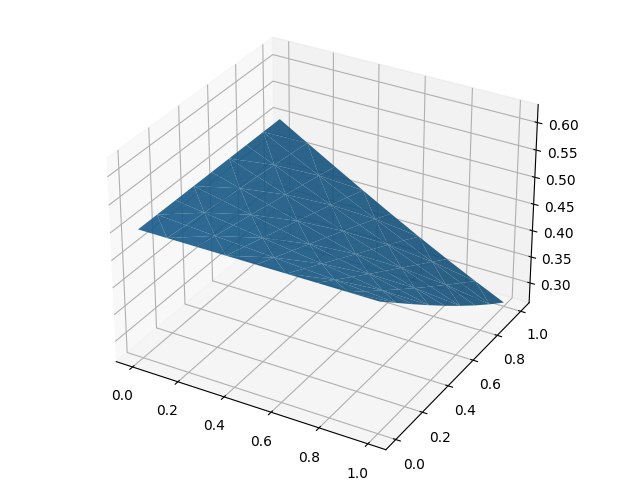
\includegraphics[width=0.3\columnwidth]{images/simple/min_surf_r3.png}
    }
    \subfigure[$ r_5(x, y)=1+\arcsin (-1+2 \sqrt{x y})$]
    {
    \centering
    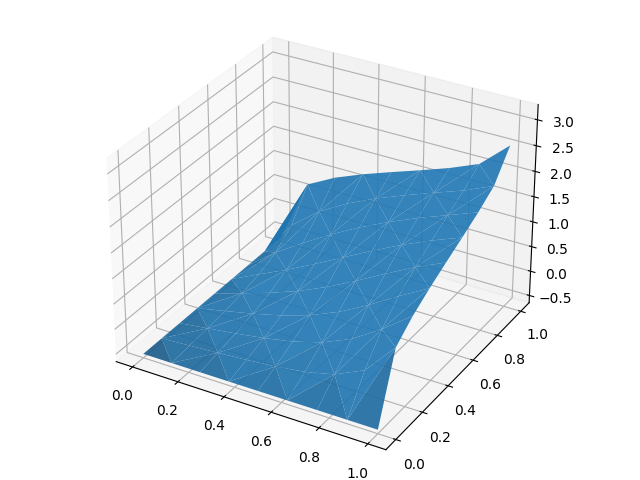
\includegraphics[width=0.3\columnwidth]{images/simple/min_surf_r4.png}
    }
    \caption{Minimum Surface Results with Five boundaries ($n=9$)}
    \label{fig:min_surf_boundaries}  
\end{figure}

\begin{figure}[!htbp]
    \centering
    \subfigure[$ r_2(x, y)$ with $n=5$]
    {
    \centering
    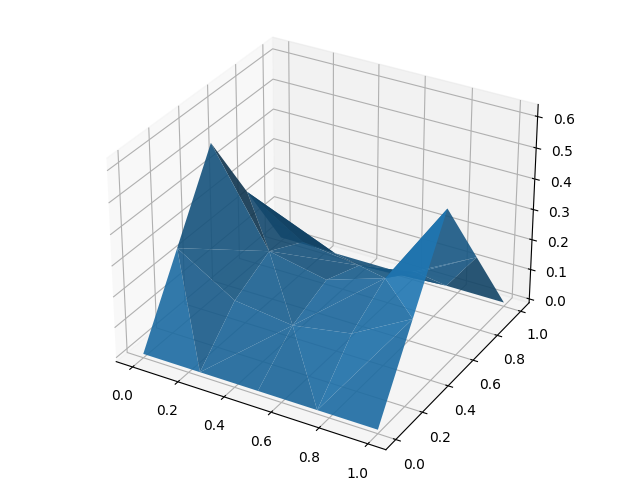
\includegraphics[width=0.3\columnwidth]{images/simple/min_surf_n5.png}
    }
    \subfigure[$ r_2(x, y)$ with $n=7$]
    {
    \centering
    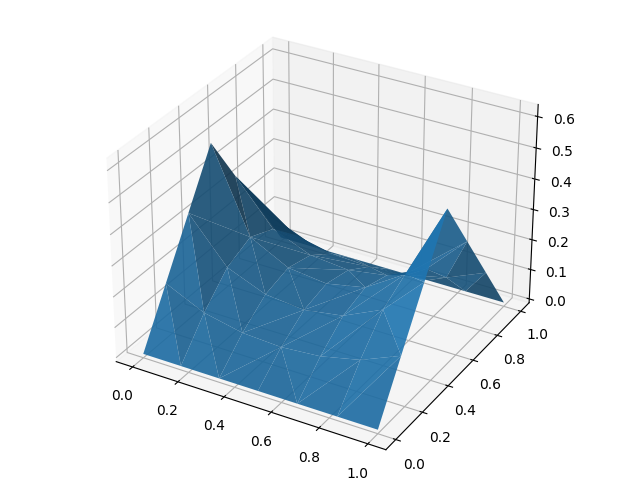
\includegraphics[width=0.3\columnwidth]{images/simple/min_surf_n7.png}
    }
    \subfigure[$ r_2(x, y)$ with $n=9$]
    {
    \centering
    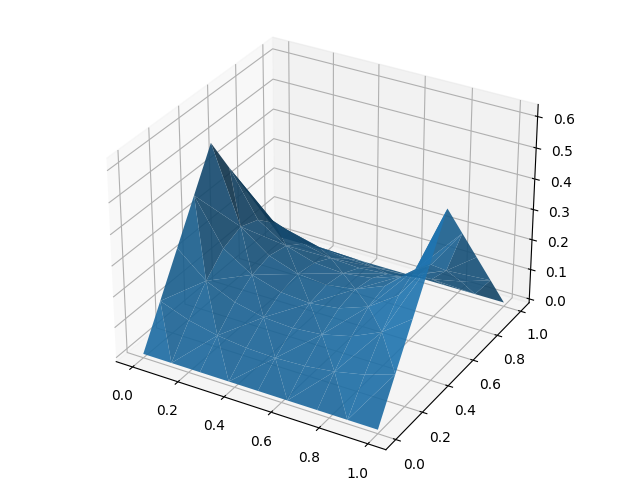
\includegraphics[width=0.3\columnwidth]{images/simple/min_surf_n9.png}
    }
    \subfigure[$ r_2(x, y)$ with $n=13$]
    {
    \centering
    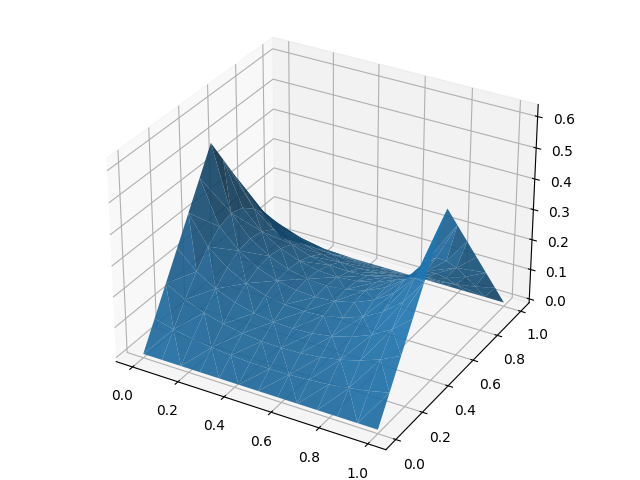
\includegraphics[width=0.3\columnwidth]{images/simple/min_surf_n13.png}
    }
    \subfigure[$ r_2(x, y)$ with $n=15$]
    {
    \centering
    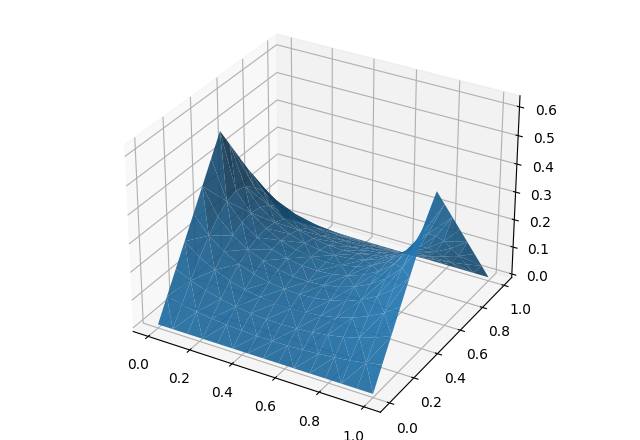
\includegraphics[width=0.3\columnwidth]{images/simple/min_surf_n15.png}
    }
    \subfigure[$ r_2(x, y)$ with $n=18$]
    {
    \centering
    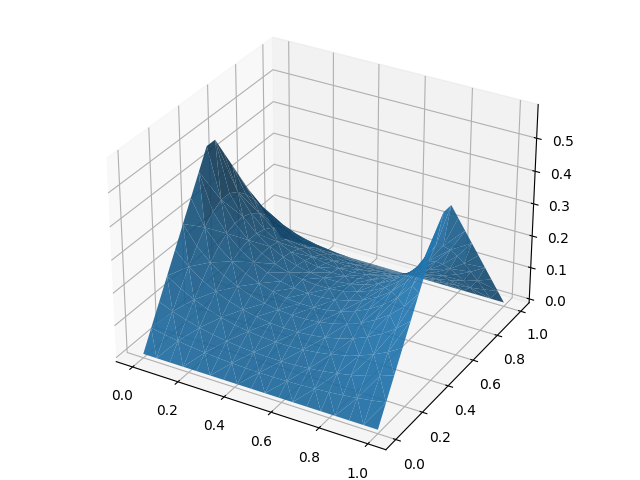
\includegraphics[width=0.3\columnwidth]{images/simple/min_surf_n18.png}
    }
    \caption{Minimum surface results with different discretization degree}
    \label{fig:min_surf_discretization}  
\end{figure}
\subsubsection{Perfomance Analysis}

In this section, we will compare the performance of the basic gradient descent method with backtracking, globalized newton method and the L-BFGS method. As we will introduce the overall performance comparison in next section, we mainly focus on the experimental results of these alogorithms via considering different discretization degree. Here, we set the boundary function $r(x, y)=\frac{1}{2}-\left|y-\frac{1}{2}\right|$. As illustrated in figure \ref{fig:alg_performance}, we can similarly conclude that the surface area becomes more smooth with larger $n$.
\begin{figure}[!htbp]
    \centering
    \subfigure[Gradient method with $n=7$]
    {
    \centering
    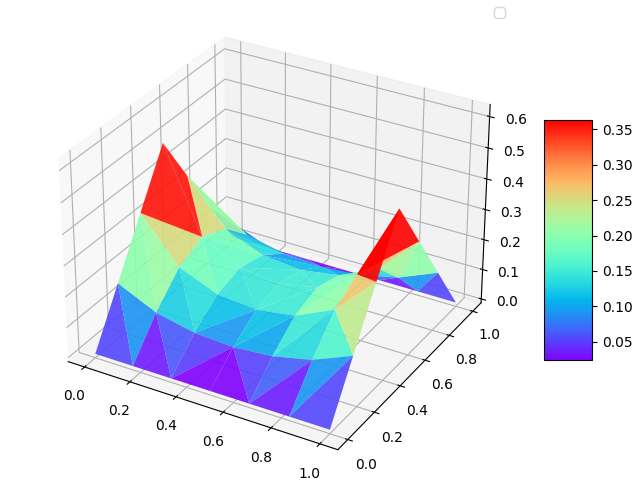
\includegraphics[width=0.3\columnwidth]{images/n_7_r_abs_ini_2/Gradient_Armijo.png}
    }
    \subfigure[Globalized newton method with $n=7$]
    {
    \centering
    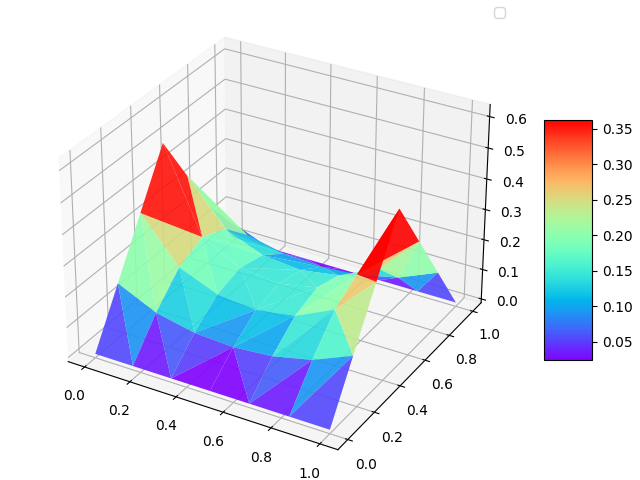
\includegraphics[width=0.3\columnwidth]{images/n_7_r_abs_ini_2/Globalized_Newton.png}
    }
    \subfigure[L-BFGS method with $n=7$]
    {
    \centering
    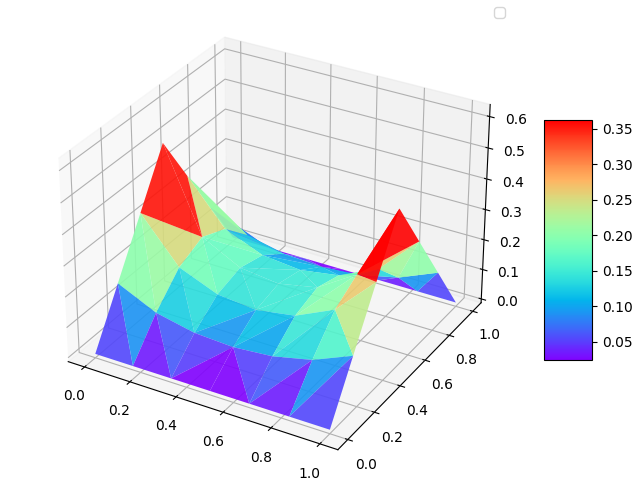
\includegraphics[width=0.3\columnwidth]{images/n_7_r_abs_ini_2/L-BFGS.png}
    }
    \subfigure[Gradient method with $n=17$]
    {
    \centering
    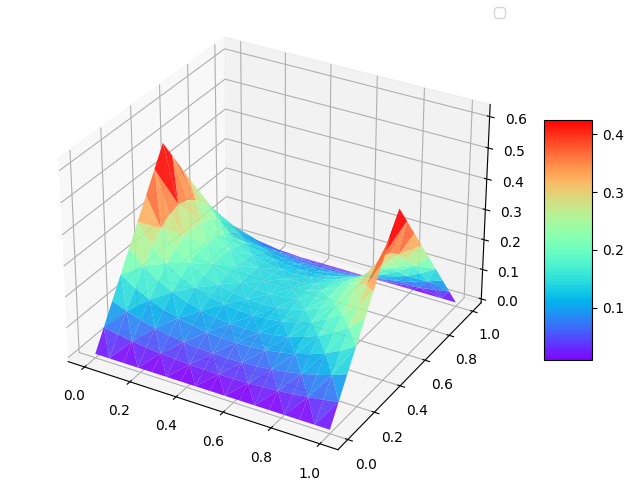
\includegraphics[width=0.3\columnwidth]{images/n_17_r_abs_ini_2/Gradient_Armijo.png}
    }
    \subfigure[Globalized newton method with $n$=17]
    {
    \centering
    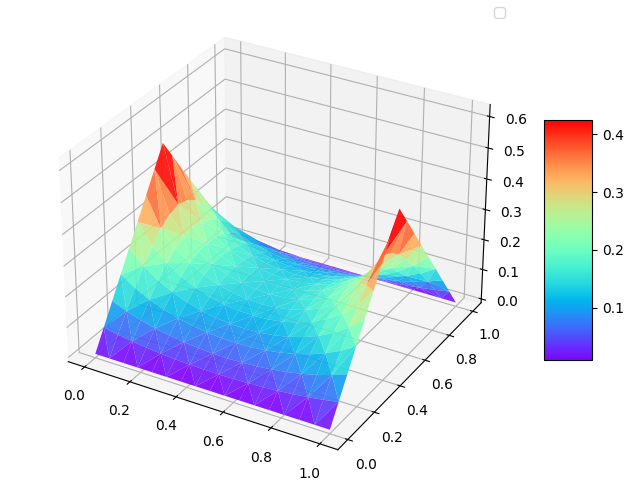
\includegraphics[width=0.3\columnwidth]{images/n_17_r_abs_ini_2/Globalized_Newton.png}
    }
    \subfigure[L-BFGS method with $n=17$]
    {
    \centering
    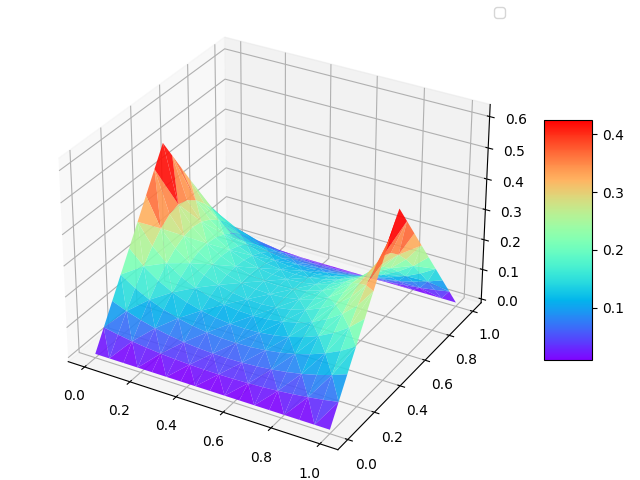
\includegraphics[width=0.3\columnwidth]{images/n_17_r_abs_ini_2/L-BFGS.png}
    }
    \caption{Minimum surface results via different algorithms with different discretization degree}
    \label{fig:alg_performance}  
\end{figure}
In table \ref{tab:per_n7} and table \ref{tab:per_n17}, we can intuitively conclude that globalized newton method perform best with the smallest iteration number and operation time while gradient method with backtracking shows the poorest performance, even though their final obejective values are very close.
\begin{table}[!ht]
    \caption{Perfomance Comparison under $n=7$}\label{tab:per_n7}
    \begin{tabular*}{\hsize}{@{}@{\extracolsep{\fill}}cccc@{}}
    \toprule
            &Iteration number  &Final objective function  &Cost time(s)  \\
    \midrule
    Gradient method   &77   &2.4514  &0.264  \\
    Globalized newton method   &5   &2.4514  &0.022  \\
    L-BFGS method   &19  &2.4514  &0.076  \\
    \bottomrule
    \end{tabular*}
\end{table}
\begin{table}[!ht]
    \caption{Perfomance Comparison under $n=17$}\label{tab:per_n17}
    \begin{tabular*}{\hsize}{@{}@{\extracolsep{\fill}}cccc@{}}
    \toprule
            &Iteration number  &Final objective function  &Cost time(s)  \\
    \midrule
    Gradient method   &780   &2.4191  &15.468  \\
    Globalized newton method   &13   &2.4194  &0.463  \\
    L-BFGS method   &46  &2.4191  &1.06  \\
    \bottomrule
    \end{tabular*}
\end{table}

\subsubsection{Additional Techniques}
In this part, we consider two more addtional techniques (exact line search and Barzilai-Borwein steps) to make comparison by the following two evalution metrics. One of the performance measures is to compare the relative objective function gap $\left|f\left(X^{k}\right)-f^{*}\right| / \max \left\{1,\left|f^{*}\right|\right\}$ with respect to the number of iterations and elapsed cpu-time. (Here $f^{*}$ denotes the optimal objective value obtained by each algorithm). Another evaluation is to compare the norm of gradients $\left(\left\|\Delta f\left(X^{k}\right)\right\|_{k}\right)$ with respect to the number of iterations and elapsed cpu-time.

In this case, we still set $r(x, y)=\frac{1}{2}-\left|y-\frac{1}{2}\right|$. When $n=17$, we can similarly get the minimum surface by the mentioned two additional techniques, as showned in figure \ref{fig:add_performance}.
\begin{figure}[!htbp]
    \centering
    \subfigure[Exact line search with $n=17$]
    {
    \centering
    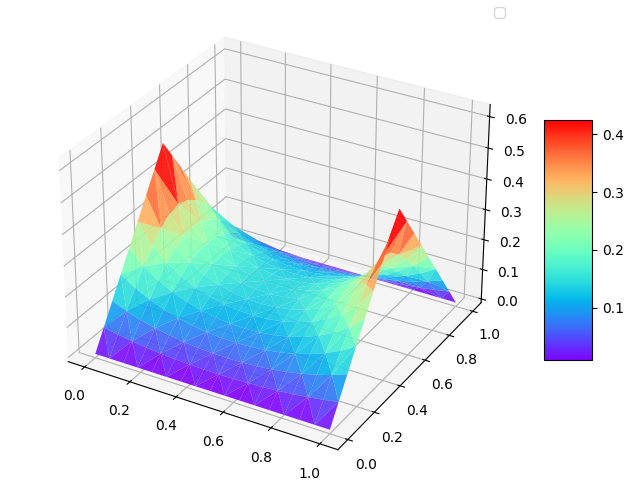
\includegraphics[width=0.42\columnwidth]{images/n_17_r_abs_ini_2/Exactline_Search.png}
    }
    \subfigure[Barzilai-Borwein steps with $n=17$]
    {
    \centering
    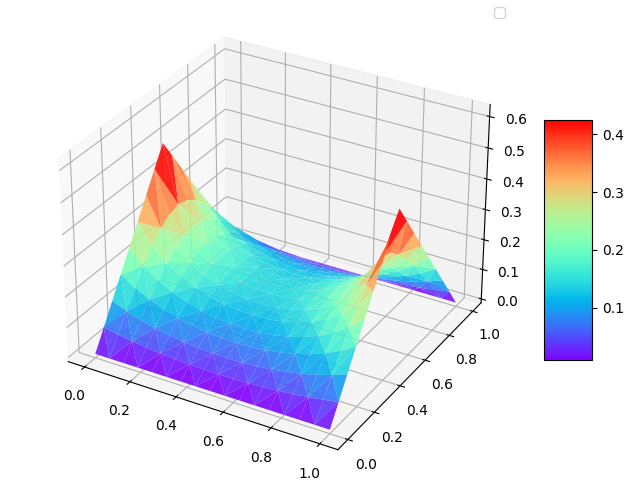
\includegraphics[width=0.42\columnwidth]{images/n_17_r_abs_ini_2/Barzilai_Borwein.png}
    }
    
    \caption{Minimum surface results via addtional techniques}
    \label{fig:add_performance}  
\end{figure}

Actually, the performance of these alogorithms vary according to our chosen performance measures. As presented in figure \ref{fig:performance_comparison}, we can demonstrate similarly that exact line search and gradient method with backtracking shows the poorer performance by analyzing the convergence curve. We can also derive a log-alogorithm to show the process of consective convergence. In figure \ref{fig:log_performance_comparison}, we can easily see the differences between different algorithms are magnified where globalized newton methods shows the best performance either from the perspective of relative objective function or norm of gradient.
\begin{figure}[!htbp]
    \centering
    \subfigure[Relative objective function gap vs number of iterations]
    {
    \centering
    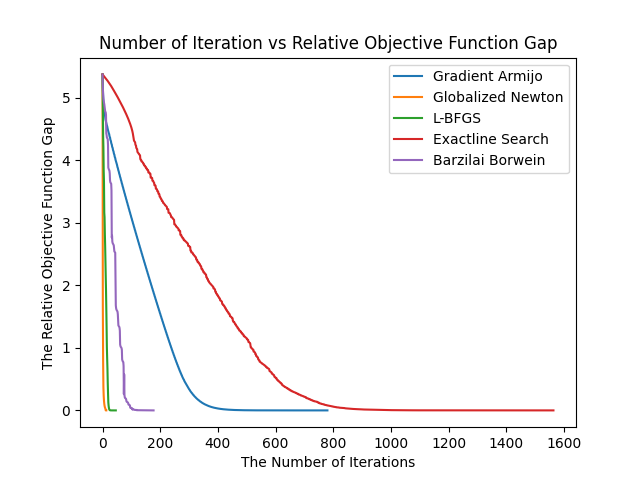
\includegraphics[width=0.42\columnwidth]{images/n_17_r_abs_ini_2/iter_gap.png}
    }
    \subfigure[Relative objective function Gap vs elapsed cpu-time]
    {
    \centering
    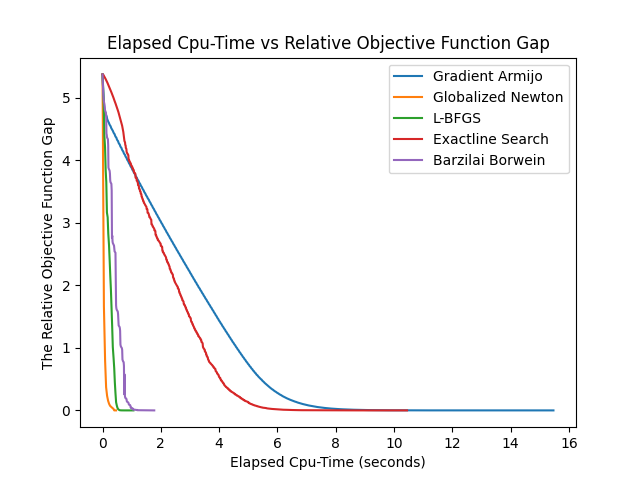
\includegraphics[width=0.42\columnwidth]{images/n_17_r_abs_ini_2/time_gap.png}
    }
    \subfigure[Norm of Gradients vs Number of Iterations]
    {
    \centering
    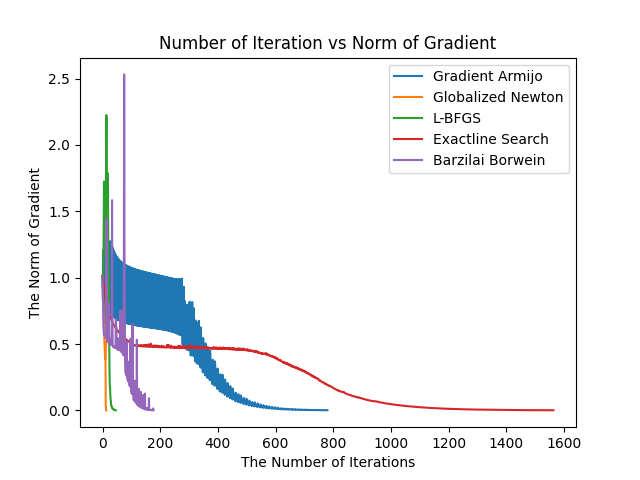
\includegraphics[width=0.42\columnwidth]{images/n_17_r_abs_ini_2/iter_g.png}
    }
    \subfigure[Norm of Gradients vs Number of Iterations]
    {
    \centering
    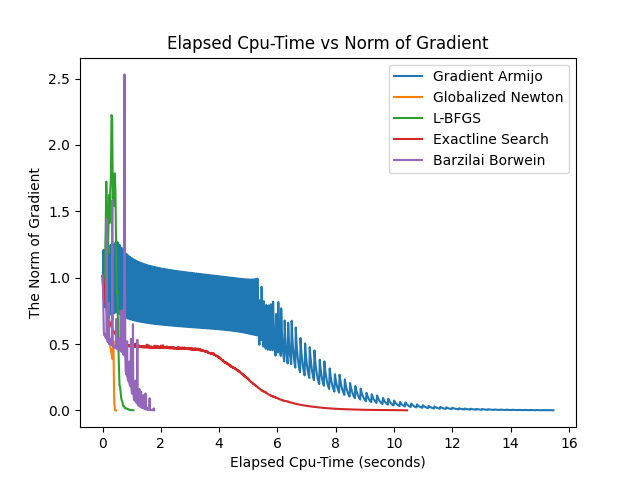
\includegraphics[width=0.42\columnwidth]{images/n_17_r_abs_ini_2/time_g.png}
    }
    \caption{Perfomance analysis via different algorithms}
    \label{fig:performance_comparison}  
\end{figure}

\begin{figure}[!htbp]
    \centering
    \subfigure[Logarithmic plot of relative objective function gap vs number of iterations]
    {
    \centering
    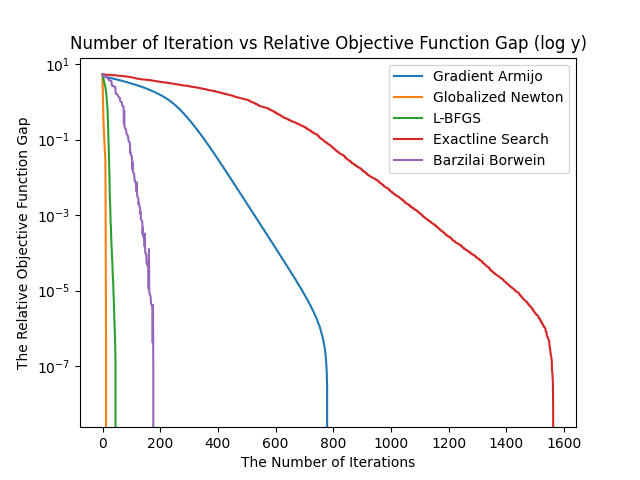
\includegraphics[width=0.42\columnwidth]{images/n_17_r_abs_ini_2/iter_gap_log_y.png}
    }
    \subfigure[Logarithmic plot of norm of gradients vs elapsed cpu-time]
    {
    \centering
    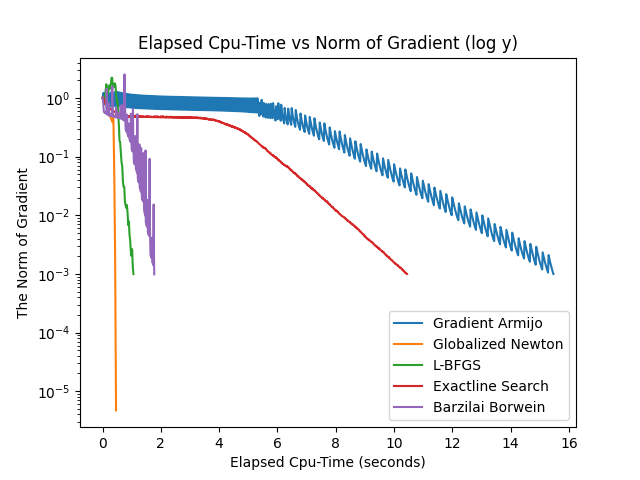
\includegraphics[width=0.42\columnwidth]{images/n_17_r_abs_ini_2/time_g_log_y.png}
    }
    \caption{Logarithmic plot of convergence performance}
    \label{fig:log_performance_comparison}  
\end{figure}
From the settings of our proposed experiments, intial points and maximum ietration number also play a vital part in the experimental results. Here, we set $n=7$ and iteration number as 20 or enough, and besides choose different intial points, to analyze how these factors influence our results. In figure \ref{fig:analysis_iteration}, it shows that exact line search method does not converge with limited iteration steps. As illustrated in figure \ref{fig:analysis_initial}, choosing different initial points can make the differences among these algorithms more obvious, where globalized newton methods still shows the best performance. 
\begin{figure}[!htbp]
    \centering
    \subfigure[Minimum surface: Exact line search with 20 iterations]
    {
    \centering
    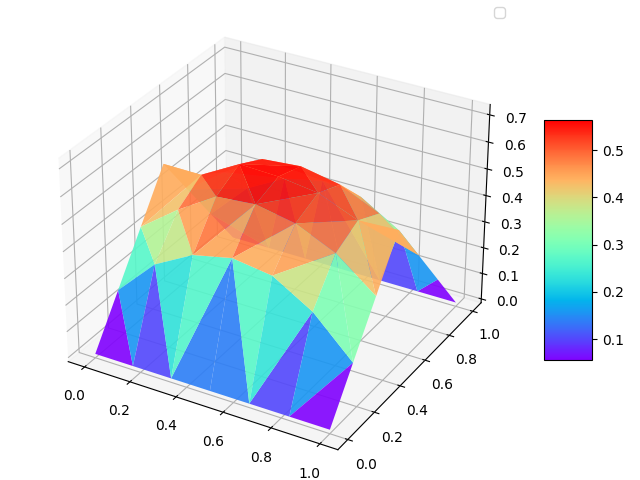
\includegraphics[width=0.45\columnwidth]{images/n_7_r_abs_ini_1/20_iter/Exactline_Search.png}
    }
    \subfigure[Minimum surface: Exact line search with enough iterations]
    {
    \centering
    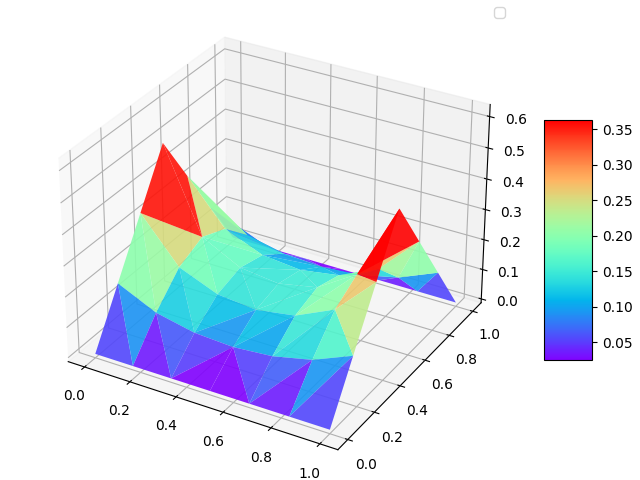
\includegraphics[width=0.45\columnwidth]{images/n_7_r_abs_ini_1/enough_iter/Exactline_Search.png}
    }
    \caption{Analysis of the influence of iteration setting}
    \label{fig:analysis_iteration}  
\end{figure}

\begin{figure}[!htbp]
    \centering
    \subfigure[Perfomance analysis with initial point 1]
    {
    \centering
    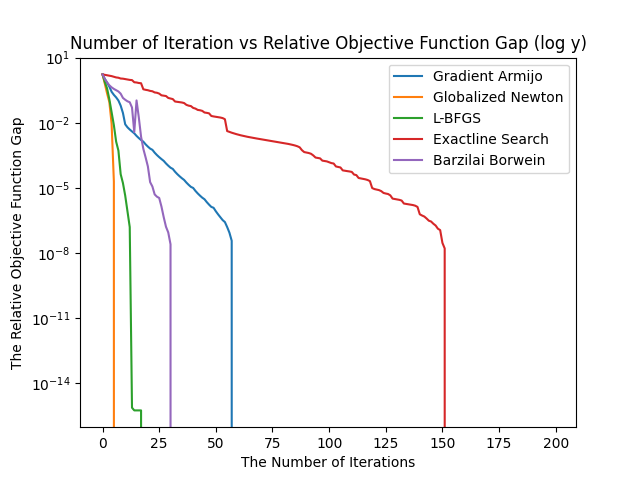
\includegraphics[width=0.42\columnwidth]{images/n_7_r_abs_ini_1/enough_iter/iter_gap_log_y.png}
    }
    \subfigure[Perfomance analysis with initial point 2]
    {
    \centering
    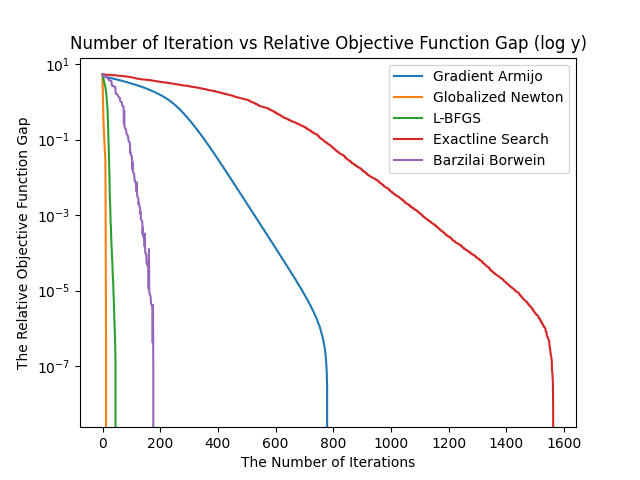
\includegraphics[width=0.42\columnwidth]{images/n_17_r_abs_ini_2/iter_gap_log_y.png}
    }
    \caption{Analysis of the influence of initial points}
    \label{fig:analysis_initial}  
\end{figure}


\subsection{Obstacle Problems}
As presented similarly in section 4.1, we firstly show different obstacles in the defiend boundary set via stochastic generation methods. We then choose projected gradient method to tackle the constrained optimization problem with different obstacle problems and illustrate corresponding minimum surface results. Lastly, We will equally present the perfomance camparing these two proposed algorithms. 
\subsubsection{Different Obstacles}
In our experiments, we generate the obstacles by designed and random methods. Figure \ref{fig:desined} shows our designed obstacles from different angle.

\begin{figure}[!htbp]
    \centering
    \subfigure[Designed generated obstacle]
    {
    \centering
    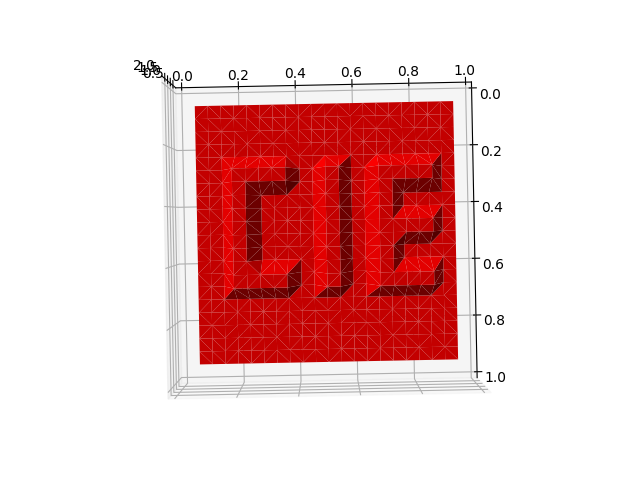
\includegraphics[width=0.42\columnwidth]{images/obstacle/origin/cie.png}
    }
    \subfigure[Designed generated obstacle]
    {
    \centering
    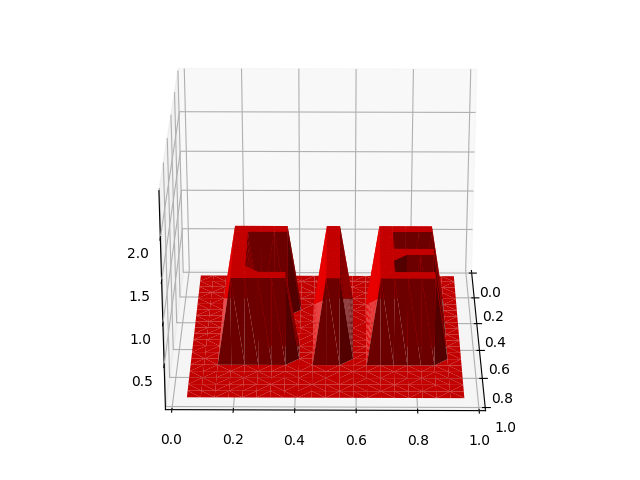
\includegraphics[width=0.42\columnwidth]{images/obstacle/origin/stochastic.png}
    }
    \caption{Illustration of designed generated obstacles}
    \label{fig:desined}  
\end{figure}

\subsubsection{Minimum Surface Results}
In this part, we will show our minimum surface results by implementing projected gradient method with five different boundary funtions. As presented in figure \ref{fig:min_des_obs} and figure \ref{fig:min_ran_obs}, we can vividly find out the process of generating minimum surfaces has been disturbed addtional obstacle constraints.
\begin{figure}[!htbp]
    \centering
    \subfigure[$ r_1(x, y)=1+\sin (2 \pi x)$]
    {
    \centering
    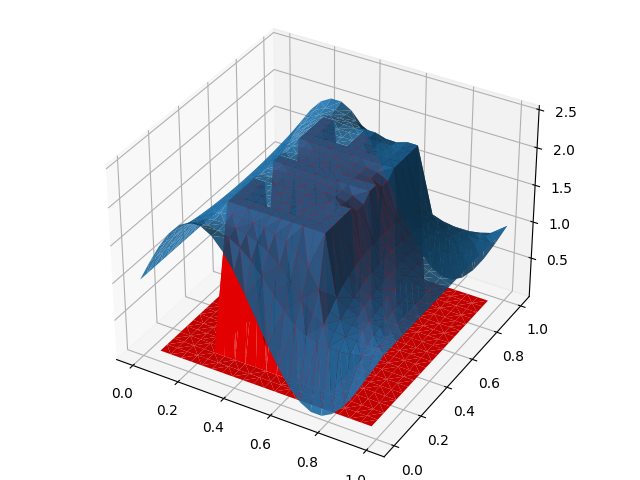
\includegraphics[width=0.3\columnwidth]{images/obstacle/cie/sin/sin_from_side.png}
    }
    \subfigure[$ r_2(x, y)=1+\cos (1 / (x+0.001) )$]
    {
    \centering
    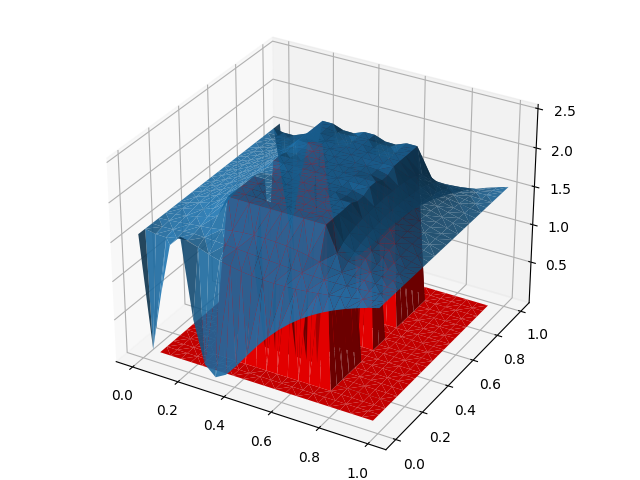
\includegraphics[width=0.3\columnwidth]{images/obstacle/cie/cos/cos_from_side.png}
    }
    \subfigure[$ r_3(x, y)=\frac{1}{2}-\left|y-\frac{1}{2}\right|$]
    {
    \centering
    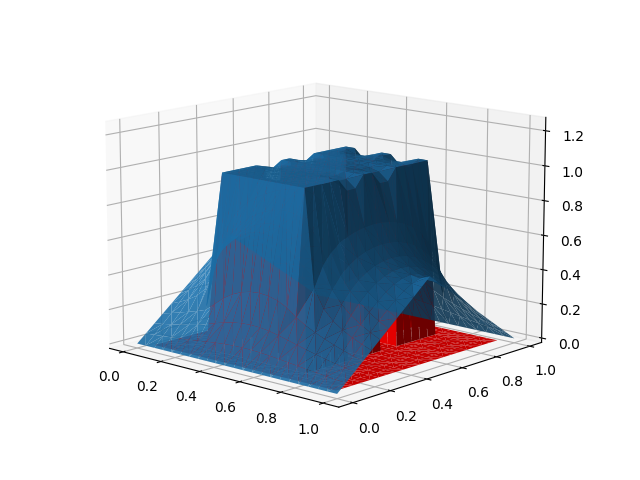
\includegraphics[width=0.3\columnwidth]{images/obstacle/cie/abs/abs_from_side.png}
    }
    \subfigure[$ r_4(x, y)=(1+\exp (x y))^{-1}$]
    {
    \centering
    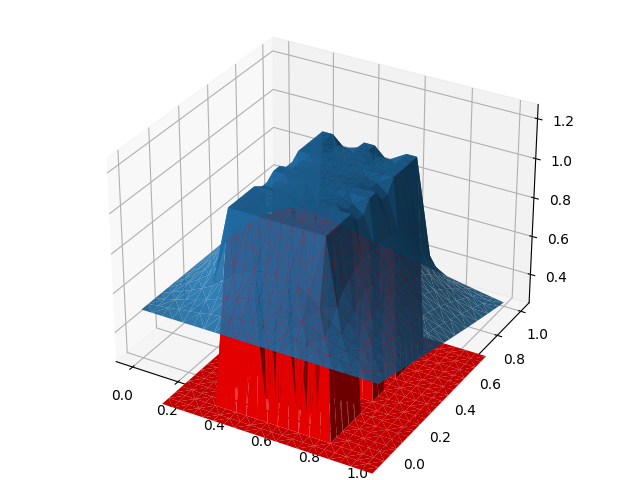
\includegraphics[width=0.3\columnwidth]{images/obstacle/cie/exp/exp_from_side.png}
    }
    \subfigure[$ r_5(x, y)=1+\arcsin (-1+2 \sqrt{x y})$]
    {
    \centering
    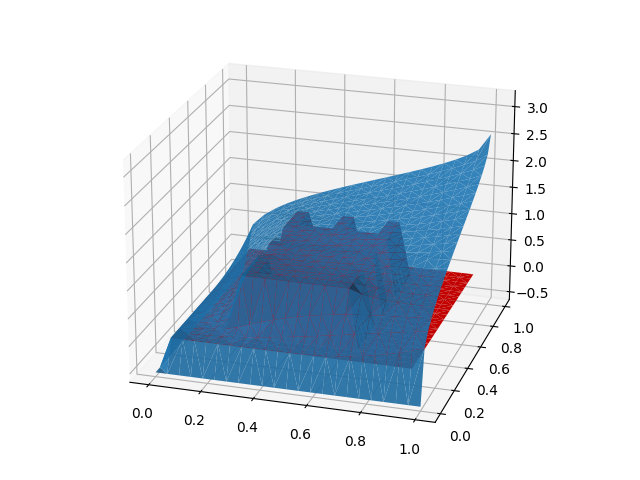
\includegraphics[width=0.3\columnwidth]{images/obstacle/cie/asin/asin_from_side.png}
    }
    \caption{Minimum Surface Results with Five Boundaries in Designed Obstacles}
    \label{fig:min_des_obs}  
\end{figure}
\begin{figure}[!htbp]
    \centering
    \subfigure[$ r_1(x, y)=1+\sin (2 \pi x)$]
    {
    \centering
    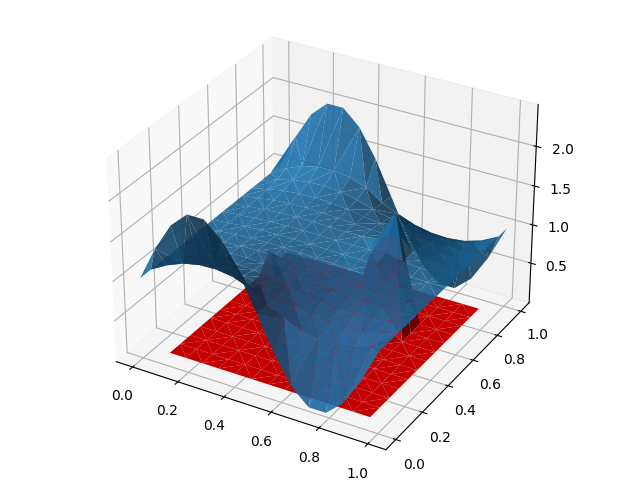
\includegraphics[width=0.3\columnwidth]{images/obstacle/random/sin/sin_from_side.png}
    }
    \subfigure[$ r_2(x, y)=1+\cos (1 / (x+0.001) )$]
    {
    \centering
    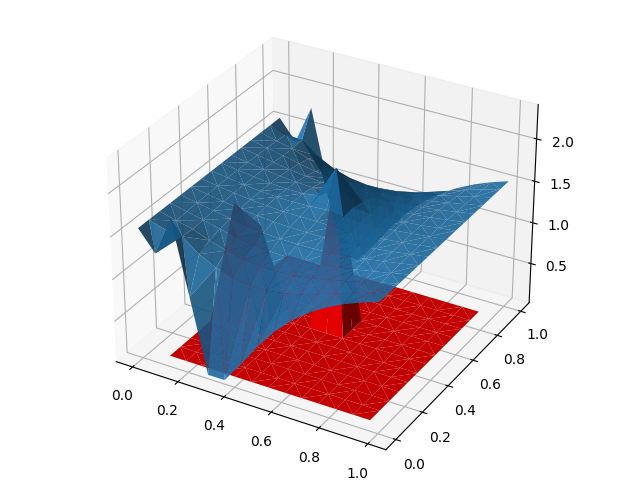
\includegraphics[width=0.3\columnwidth]{images/obstacle/random/cos/cos_from_side.png}
    }
    \subfigure[$ r_3(x, y)=\frac{1}{2}-\left|y-\frac{1}{2}\right|$]
    {
    \centering
    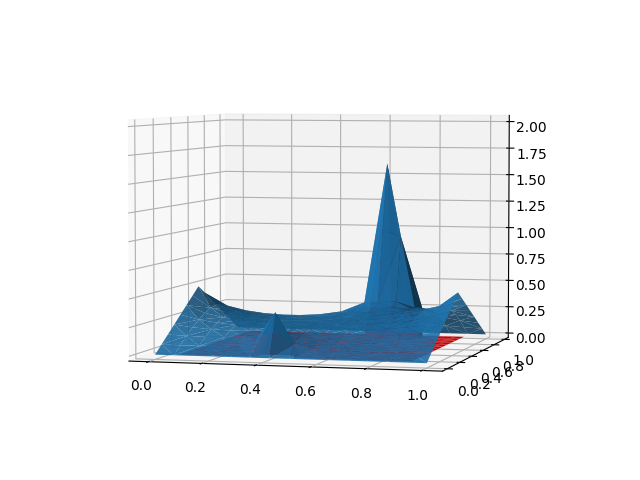
\includegraphics[width=0.3\columnwidth]{images/obstacle/random/abs/abs_from_side.png}
    }
    \subfigure[$ r_4(x, y)=(1+\exp (x y))^{-1}$]
    {
    \centering
    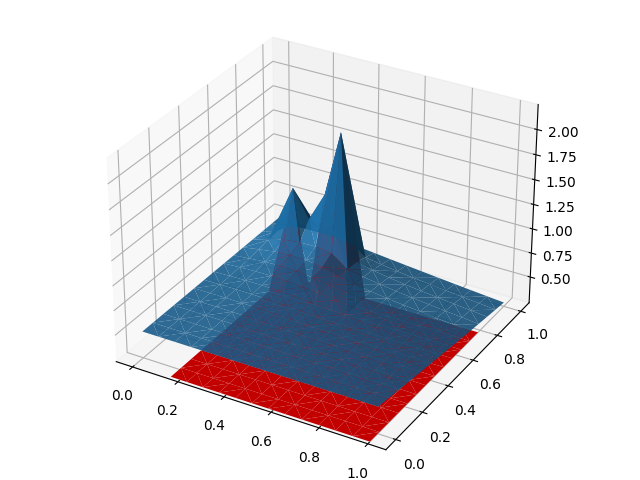
\includegraphics[width=0.3\columnwidth]{images/obstacle/random/exp/exp_from_side.png}
    }
    \subfigure[$ r_5(x, y)=1+\arcsin (-1+2 \sqrt{x y})$]
    {
    \centering
    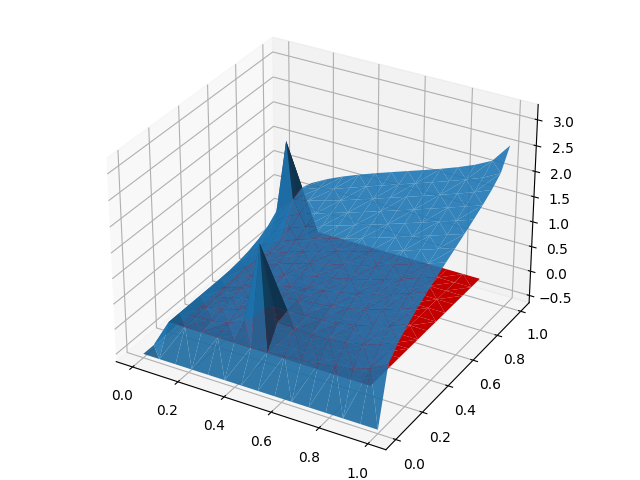
\includegraphics[width=0.3\columnwidth]{images/obstacle/random/asin/asin_from_side.png}
    }
    \caption{Minimum Surface Results with Five Boundaries in Random Obstacles}
    \label{fig:min_ran_obs}  
\end{figure}

\subsubsection{Perfomance Analysis}
Here we use the quadratic penalty method and the projected gradient armijo
method to solve the minimal surface problems with designed obstacles. Table \ref{tab:qua} shows one of the comparison results with the boundary funtion $ r_3(x, y)=\frac{1}{2}-\left|y-\frac{1}{2}\right|$. It can easily find that quadratic penalty method shows worse performance compared with projected gradient method with higher iteration number and operation time. This is because when implementing the penalty method, it needs a sub method to minimize the penalty function, which causes more iterations to converge and takes more operation time.
\begin{table}[!ht]
    \caption{Perfomance comparison between quadratic penalty method and projected gradient method}\label{tab:qua}
    \begin{tabular*}{\hsize}{@{}@{\extracolsep{\fill}}cccc@{}}
    \toprule
            &Iteration number  &Final objective function  &Cost time(s)  \\
    \midrule
    Projected gradient method    &784   &5.45  &19.18  \\
    Quadratic penalty method  &873   &5.45  &123.17  \\
    \bottomrule
    \end{tabular*}
\end{table}

\section{Discussion}
\subsection{Main Experimental Observations}
In the process of our experiment, we found that besides the property of different optimality solving method, the way of implementation could largely influence the speed. For example, using \textit{C} or \textit{Matlab} could be usually faster than \textit{Python} especially in the case that there are multi-layers loops, while it's quite common in the methods we study.

The other important factor we found that could influence the speed is the process of taking gradient and hessian. If we use the \textbf{auto-gradient toolkit}, it would be the slowest since every time it will use the \textbf{computational graph}, which is a data structure that can largely influence the speed. For the \textbf{symbolic-gradient toolkit}, we have most of our time-cost at the process of getting the expression. After such process, the calculation speed will be much faster than that of the auto-gradient method. However, this would still cause some problems. First, it's not so convenient that when $n$ changes, we need to recaculate the symbolic expression. Second, when $n$ is very large, and consider that the hessian would be very sparse, the evaling process will be very slow. Manually get the gradient and hessian expression and define corresponding function in the program would be the fastest way, but we will then lose some flexibility while it's well specified.

One simple way that we can improve the speed in the Minimal Surface problem is to utilize the optimal surface share the same \textbf{symmetry} as that of the boundary. For example, we know that for the boundary generated by $r_3(x,y) = \frac{1}{2} - |y - \frac{1}{2}|$ and $\Omega = (0,1) \times (0,1) \in R^2$ , $\Gamma=\partial \Omega$, we will have $f(\frac{1}{2}-x)=f(\frac{1}{2}+x)$ as well as $f(\frac{1}{2}-y)=f(\frac{1}{2}+y)$, so we can reduce the number of decision variables by $\frac{3}{4}$ as long as we maintain these two equations.

Finally, we would like to say that good \textbf{isolation and encapsulation} of our codes help us to carry out experiments more efficiently. You can utilize any instance that is a subclass \texttt{Solver} and use its implemented \texttt{solve} function to solve an instance that is a subclass of \texttt{Solver}. In the implementation of the quadratic penalty method, we even let our solver hold the reference of an Armijo Gradient Method. You can check the code on \textbf{Github}\footnote{\url{https://github.com/WhiskyChoy/opt_final_project}} and initialize any problem or solver as you wish.

\subsection{Extensions and Applications}
As indicated in paper \cite{yueting2007compact}, the compact form of L-BFGS is more efficient to adapt for sparse cases. Moreover, the compact form has an analog for the direct update. The compact representation of the quasi-Newton updating matrix is derived to the use in the form of limited memory update in which the vector is replaced by a modified vector so that more available information about the function can be employed to increase the accuracy of Hessian approximations. The global convergence of the proposed method is also proved \cite{yueting2007compact}. It’s expected that the compact form of the L-BFGS can provide a new model for solving more kinds of large scale optimization. 

Besides, for the existing problems in this project, we may consider more advance and sufficient algorithms to solve the defined minimum surfaces and obstacle problems, such as applying augmented-lagrange method to modify the performance of penalty parameter and Alternating Direction Method of Multiplier (ADMM) where alternate minimization are utilized to decouple sets of variables that are coupled within the augmented Lagrangian.

We can also extand our problems to a more common case. For instance, we assume that obstacle can move freely within the target set and determine what is the maxmimum minimal area. This general problem can be solved by 
sequential quadratic programming. Considering paper \cite{caffarelli2016obstacle}, the authors also discuss the regularity of the solution and of the free boundary for certain obstacle type problems involving classical minimal surfaces and nonlocal minimal surfaces, which can be further investigated.

Furthermore, in \cite{attouch2014variational}, researchers have pointed out several application scenerios such as fluid filtration in porousmedia, constrained heating, elasto-plasticity and optimal control. Since the obstacle problem has some potential physical meaning, we may considering combining additional physical definition to solve the pracitical obstacle problems.

\section{Conclusion}




\bibliographystyle{unsrt}
\bibliography{refs}
\end{document}
